\documentclass{article}

% Language setting
%\usepackage[english]{babel}

% Set page size and margins
% Replace `letterpaper' with `a4paper' for UK/EU standard size
\usepackage[letterpaper,top=2cm,bottom=2cm,left=3cm,right=3cm,marginparwidth=1.75cm]{geometry}

% Useful packages
\usepackage{amsmath}
\usepackage{graphicx}
\usepackage[colorlinks=true, allcolors=blue]{hyperref}
\usepackage{rotating}
\usepackage{graphicx}

\title{GEO 242 Final Project: Repeater-derived creep rates for the Hayward Fault}
\author{Norma A. Contreras}
\date{December 02, 2022}

\begin{document}
\maketitle

\section{Introduction}
For this project I attempted to estimate short- and long-term creep rates for the Hayward fault in California. Repeaters were identified using the Fully-Automated Repeating Earthquake Search (FARESearch) code, using data from the Northern California Earthquake Data Center (NCEDC) \cite{funning21,ncedc}. The Hayward fault was selected for this project for two main reasons: existing confirmation of creep along the fault, with some studies exploring its creep rate over a century \cite{lienkaemper91}, and the tentative results produced by FARESearch. A search for repeaters was conducted on nearby faults, but the Hayward produced the most practical results for the scope of this project. Other faults, such as the Calaveras (included in the southern portion of the selected study area, see Fig.\ref{fig:creep_locs}), produced over forty grids and was not selected due to complications relating to repeater identification in select grids. Faults such as the Rodgers Creek fault, produced fewer grids (i.e. four or less) and had significantly fewer repeaters. 

\section{Repeating earthquakes on the Hayward fault zone}
\subsection{FARESearch results}
FARESearch divided the selected fault polygon into fourteen grids, identifying $\sim$6,000 events as repeaters, fewer than the results obtained by Funning and Shakibay Senobari \cite{funning21}. These events were separated into $\sim$1,015 repeater sequences. It is important to note that the southern portion of the selected polygon included portions of the Calaveras fault, resulting in the "contamination" of repeater sequences. 

\begin{figure}
\centering
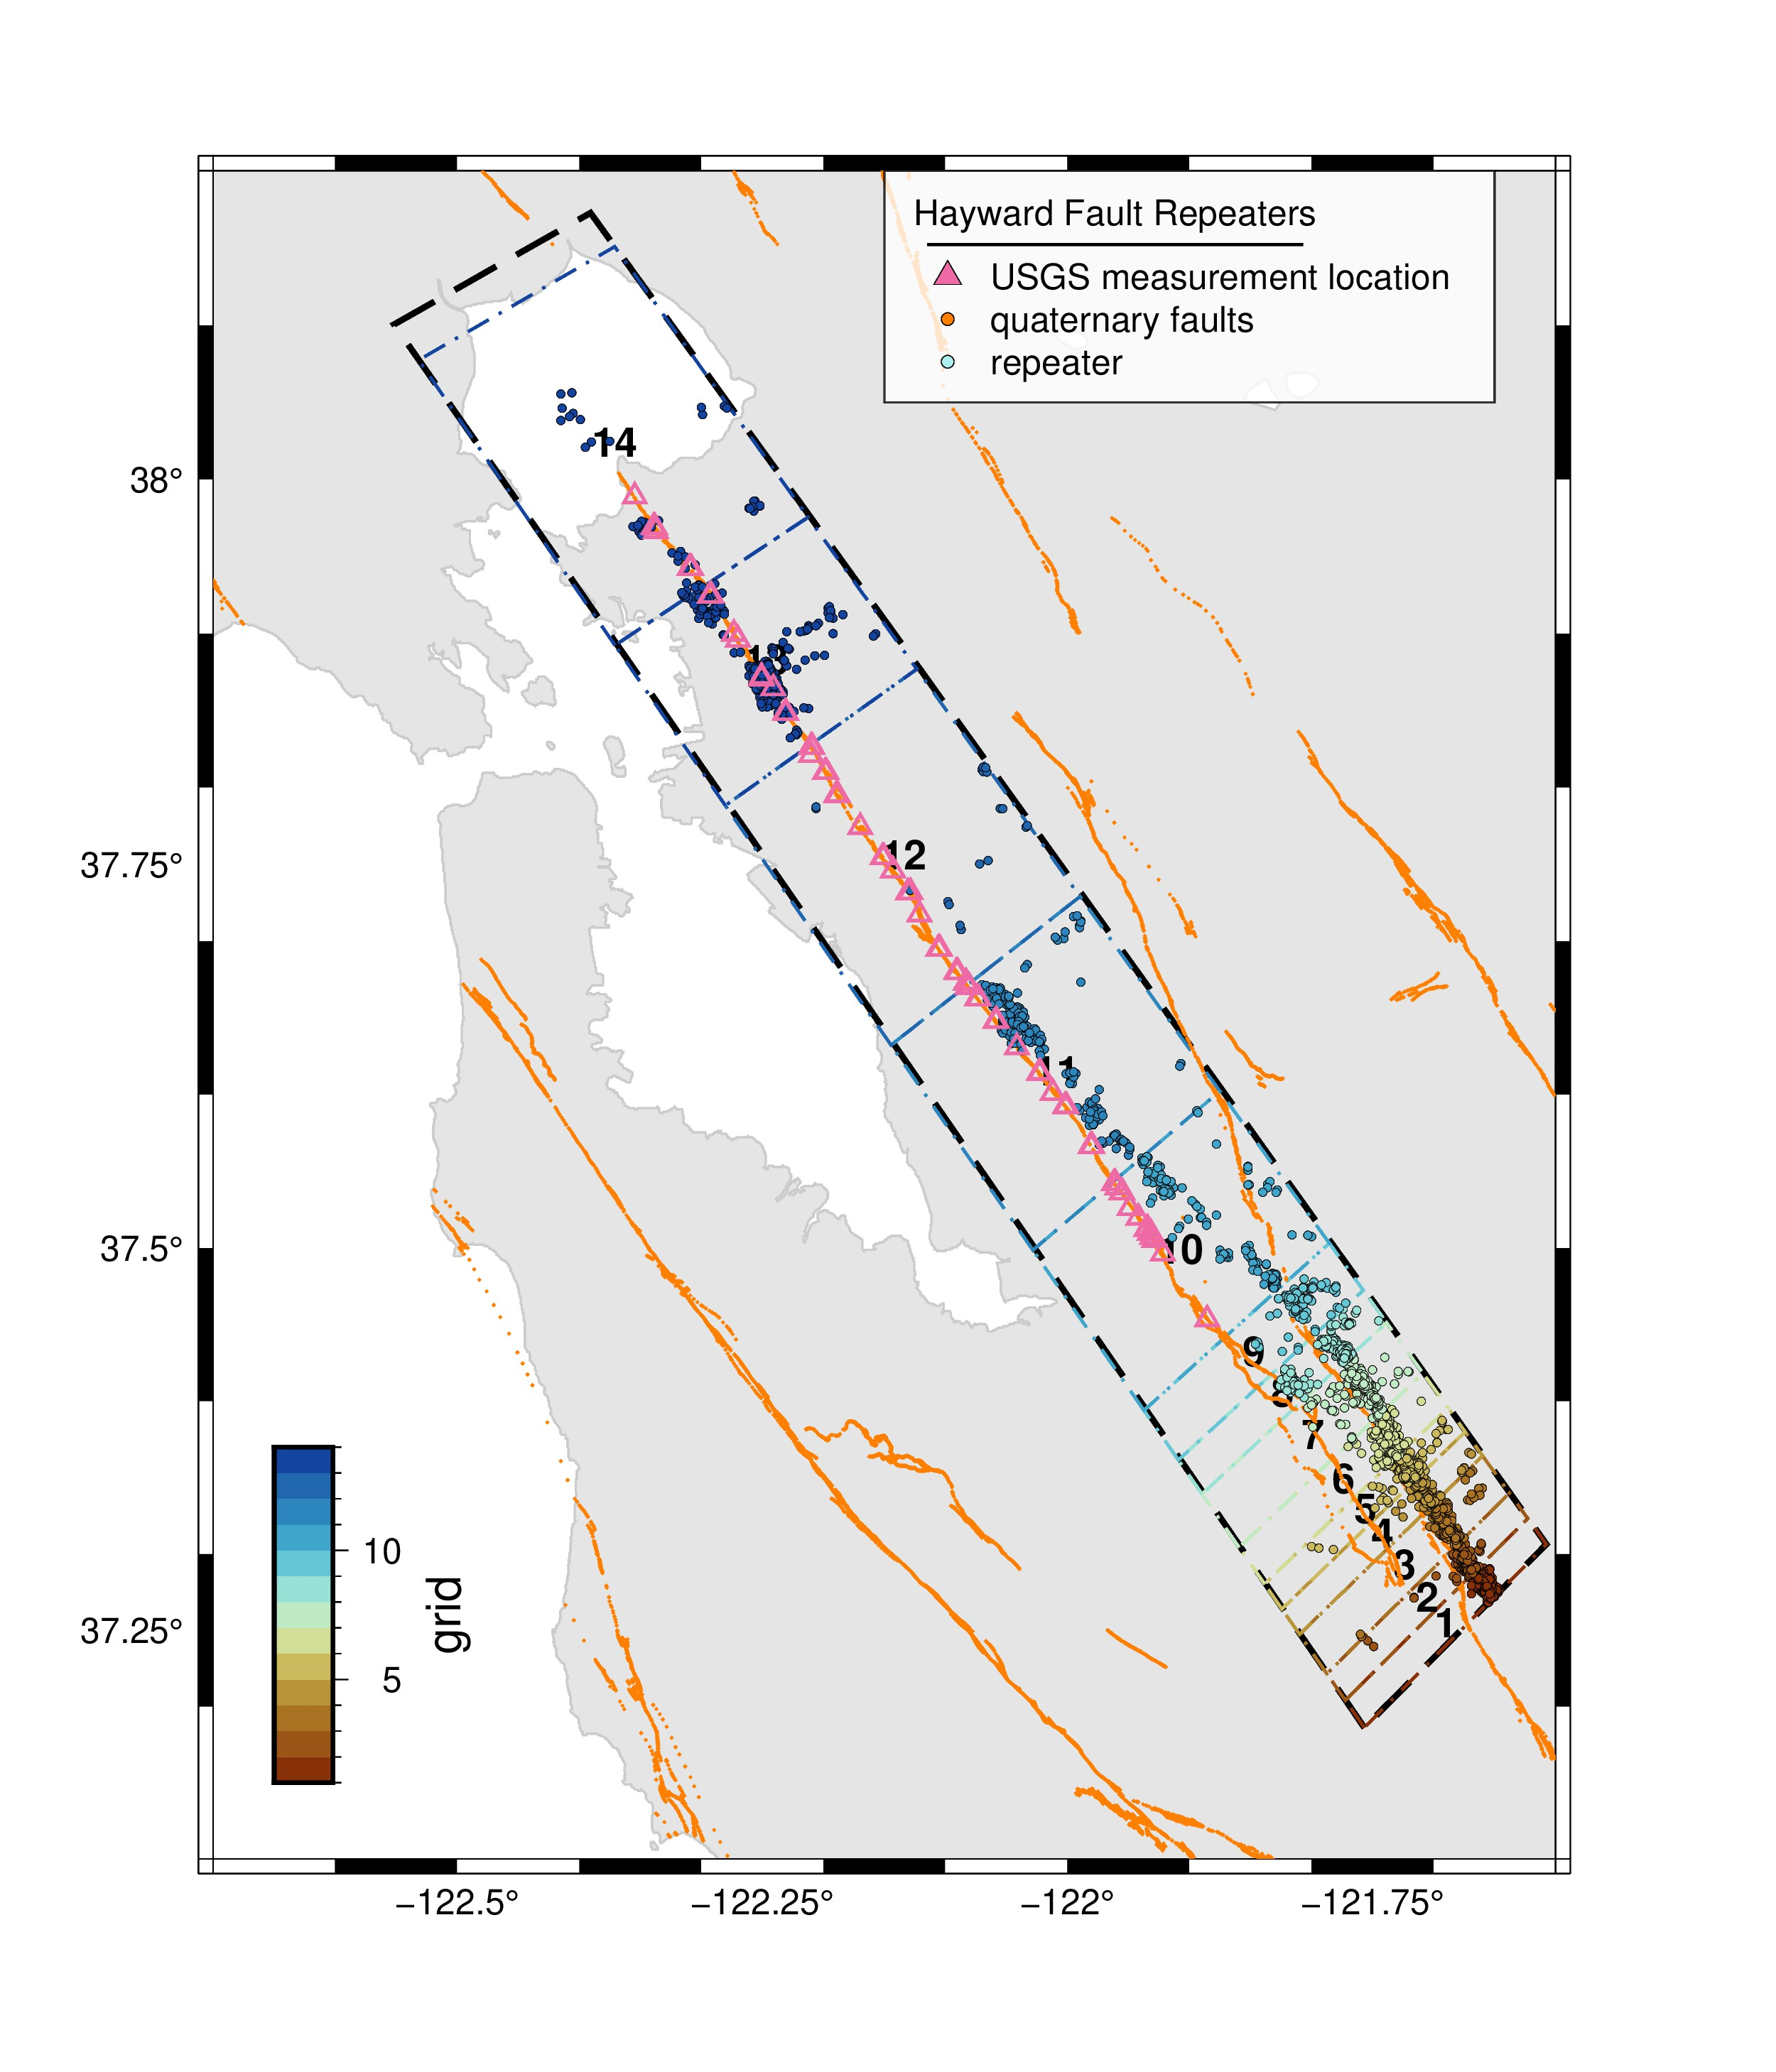
\includegraphics[height=7.25in]{creep_locs.jpg}
\caption{\label{fig:creep_locs}Complete catalog of repeating earthquakes identified by FARESearch. The locations of USGS surface creep rate measurements taken is plotted as well \cite{johnson22}. Repeating events are color coded based on the grid they are located on for easy identification.}
\end{figure}

Following the example set by Chen et al. \cite{chen08}, consecutive events with recurrence intervals less than 0.1 years were filtered out, leaving $\sim$900 repeater sequences. This resulted in the elimination of various doublets. A potential issue arose when two consecutive events in the middle of a sequence had recurrence intervals that did not meet the minimum value. Events immediately before and after kept the recurrence intervals calculated. In essence,
\newline
\newline
For a sequence we have $N$ events with times $t$:
\begin{equation}
[t_1, t_2, t_3, t_4, ... t_N]
\label{eq:time_evs}
\end{equation}

We then have $N-1$ recurrence intervals, $T_r$:
\begin{equation}
    [(t_2 - t_1), (t_3 - t_2), (t_4 - t_3),..., (t_N - t_{N-1})] =  [Tr_1, Tr_2, Tr_3, Tr_4, ..., Tr_N]
    \label{eq:Tr}
\end{equation}

If $Tr_2 < 0.1$ years, it was removed from the recurrence interval array,  leaving:
\begin{equation}
    [Tr_1, Tr_3, Tr_4, ... Tr_N] =
    [(t_2 - t_1), (t_4 - t_3),..., (t_N - t_{N-1})]
    \label{eq:Tr_filter}
\end{equation}
Where events $t_3$ and $t_2$ were still referenced by $Tr_1$ and $Tr_3$.
In addition to this issue, several repeater sequences were reduced to pairs of events, or eliminated completely, resulting in some grids containing few repeater sequences (Fig.\ref{fig:slip}).

\section{Slip parameter calibrations}
Nadeau and Johnson derived the following relationship between the slip and seismic moment of repeater sequences using repeaters from the Parkfield portion of the San Andreas fault \cite{nadeau98,nadeau04}.
\begin{equation}
    log(d) = \alpha_d + \beta_d log(M_0)
    \label{eq:slip_M0}
\end{equation}

or:
\begin{equation}
    d_i = 10^\alpha_d M_0 ^\beta
    \label{eq:slip_M0_2}
\end{equation}

Where $d$ and $M_0$ have units cm and dyne-cm, respectively. Their estimated $\alpha_d$ and $\beta_d$ values are:
\begin{equation}
    \alpha_d = -2.36; \beta_d = 0.17
    \label{eq:parkfield_const}
\end{equation}
Chen et al. provide equations for short- and long-term creep rates for a repeater sequence, derived from Eqn. \ref{eq:slip_M0}\cite{chen08}:
\begin{equation}
    V_d(i) = \frac{\sum_{i=2}^{N} d_i}{\sum_{j=1}^{N-1} T_r(i)}
    \label{eq:Vd_short}
\end{equation}

\begin{equation}
    V_d = \frac{\sum_{i=1}^{N} d_i}{T_obs}
    \label{eq:Vd_long}
\end{equation}
Where, $V_d(i)$ is the short-term creep rate, $V_d$ is the long-term creep rate, $i$ is the repeater event, $T_obs$ is the observation period, $j$ is the recurrence interval, and $N$ is the total number of events for a sequence.

Eqn. \ref{eq:slip_M0} has been used in various studies, with varying degrees of success using the Parkfield parameters \cite{shakibay19,khoshmanesh15,chen08,igarashi03,matsuzawa02}; We will explore the applicability of these constants to the Hayward fault.

\subsection{$\beta_d$ calibrations}
We will start by using the relationship between the recurrence interval, $T_r$, and seismic moment, $M_0$, of repeaters \cite{nadeau98,chen07}:
\begin{equation}
    log(T_r) = \alpha_T + \beta_T log(M_0)
    \label{eq:Tr_M0}
\end{equation}

Where $T_r$ and $M_0$ have units in seconds and dyne-cm, respectively. Nadeau and Johnson's estimated $\alpha_T$ and $\beta_T$ values are:
\begin{equation}
    \alpha_T = 4.85; \beta_T = 0.17
    \label{eq:parkfield_const_Tr}
\end{equation}

The slip parameter, $\beta_d$, is approximately equal to $\beta_T$ \cite{nadeau98}. We take advantage of this, using Eqn.\ref{eq:Tr_M0} to estimate the $\beta_d$ constant. Before doing so, we calculate the recurrence intervals using seconds, and convert the NCEDC magnitudes ($M_d$) into seismic moment using the relationship derived by Bakun for central California \cite{bakun84}:
\begin{equation}
    log(M_0) = 1.2 M_d + 17
    \label{eq:md_conversion}
\end{equation}

To fit $\beta_T$, we use Eqn.\ref{eq:Tr_M0}, setting up a linear system of equations of the form:
\begin{equation}
    \begin{bmatrix}
        log(M0_{i1}) & 1 \\
        log(M0_{i2}) & 1 \\
        ...
    \end{bmatrix} 
    \begin{bmatrix}
        \beta_T \\
        \alpha_T
    \end{bmatrix}
    =
    \begin{bmatrix}
        log(Tr_{i1})\\
        log(Tr_{i1})\\
        ...
    \end{bmatrix}
    \label{eq:lsq_mx}
\end{equation}

where the seismic moment and recurrence interval matrices are populated by the log of the average values of each repeater sequence ($T_r \geq 0.1 yrs$). We solve for this using a least squares fit, and find:
\begin{equation}
    \alpha_T = 2.6529;
    \beta_T = 0.2831 = \beta_d
    \label{eq:LSQ_const_Tr}
\end{equation}

\begin{figure}
\centering
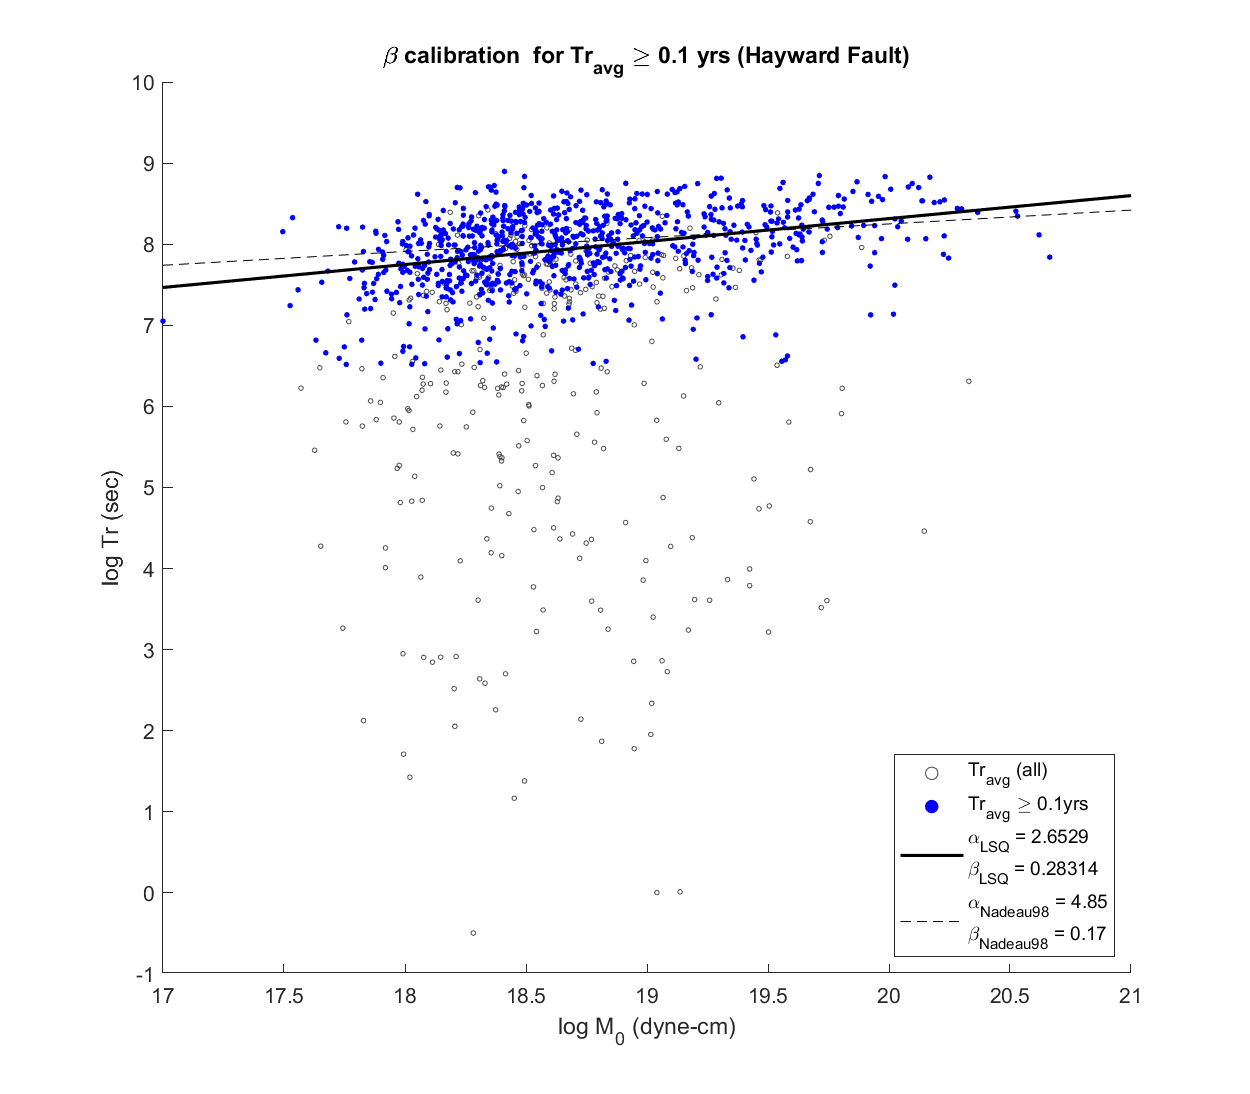
\includegraphics[width=4.5in]{Tr_M0_comparison.png}
\caption{\label{fig:TrM0} Least squares fitting for recurrence interval $T_r$ and seismic moment, $M_0$. Our $\alpha_T$ is roughly half that of Nadeau and Johnson, while our $\beta_T$ is roughly twice their $beta_T$ value. We only use recurrence intervals greater than or equal 0.1 years for the fitting.}
\end{figure}

\subsubsection{Jackknife analysis of $\beta_T$}
The jackknife resampling method is applied to the $\beta_T$ estimate. During each interation, one repeater sequence is removed, and the $\beta_T$ and $\alpha_T$ constants are recalculated. Fig.\ref{fig:jackknife} shows the results for the $\beta_T$ parameter calculations. 

\begin{figure}
\centering
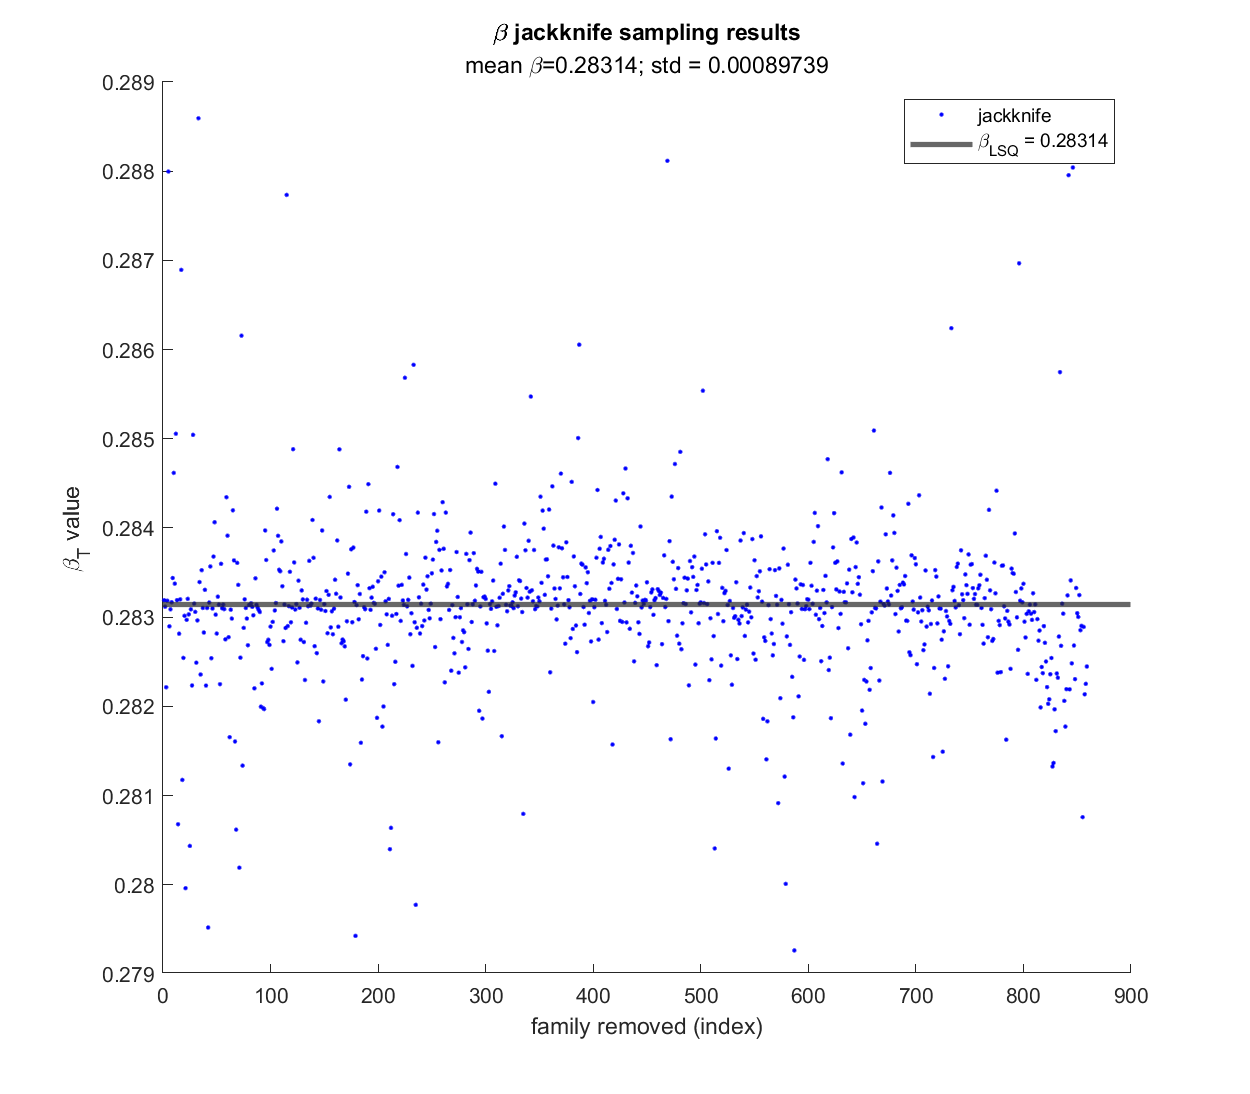
\includegraphics[width=4.5in]{jackknife_results.png}
\caption{\label{fig:jackknife} Jackknife sampling of the least squares fit for $\beta$. Consecutive repeater events with a recurrence interval less than 0.1 years were removed prior to the calibration.}
\end{figure}

\subsection{$\alpha_d$ calibrations}
To solve for $\alpha_d$ we use the following relationship from Nadeau and Johnson \cite{nadeau98}:
\begin{equation}
    \alpha_T = \alpha_d - log(\dot{\tilde{d}})
    \label{eq:alpha_TD}
\end{equation}
Where $\dot{\tilde{d}}$ is the average rate of slip. 

To calculate the average rate of slip, we use surface creep rates from the 2023 USGS creep rate model for California faults \cite{johnson22}. Shakibay Senobari and Funning calibrated the $alpha_d$ constant for the Rodgers Creek fault using a shallow repeater sequence and the InSAR surface creep rate for that area \cite{shakibay19}. A similar protocol is followed here. By overlaying the USGS measurement locations with our initial FARESearch repeater events (Fig.\ref{fig:creep_locs}), we can see that grid thirteen has events that align well with the available USGS measurement locations. We calculate the USGS average surface creep rate for this grid and use this in Eqn.\ref{eq:alpha_TD} to solve for $\alpha_d$. Note that $\dot{\tilde{d}}$ is presented in cm/year here for clarity; the calculations were carried out using units of cm/sec.

\begin{equation}
    \dot{\tilde{d}} = 0.3963 (cm/yr);
    \alpha_d = -5.2479
\end{equation}

\section{Slip and creep estimations}
Having calculated $\alpha_T$, $\alpha_d$, $\beta_T$ ($=\beta_d$), and recurrence intervals, we can calculate slip and creep rates from Eqns. \ref{eq:slip_M0_2}, \ref{eq:Vd_short}, and \ref{eq:Vd_long}. Our results are shown in Figs.\ref{fig:slip} (slip), \ref{fig:Vd_short} (short-term creep rate), and \ref{fig:Vd_long} (long-term creep rate). We compare the slip and creep-rates for three different calibrations:
\newline
Khoshmanesh \cite{khoshmanesh15}: 
\begin{equation} \alpha_d = -1.56; \beta_d = 0.1 \end{equation}
\newline
Nadeau \cite{nadeau98}: \begin{equation}\alpha_d = -2.36; \beta_d = 0.17\end{equation}
\newline
Ours: \begin{equation}\alpha_d = 5.2479; \beta_d = 0.28314\end{equation}

Overall, our $\alpha_d$ and $\beta_d$ constants produced consistently lower values that failed to fit the available USGS data.

\begin{sidewaysfigure}
    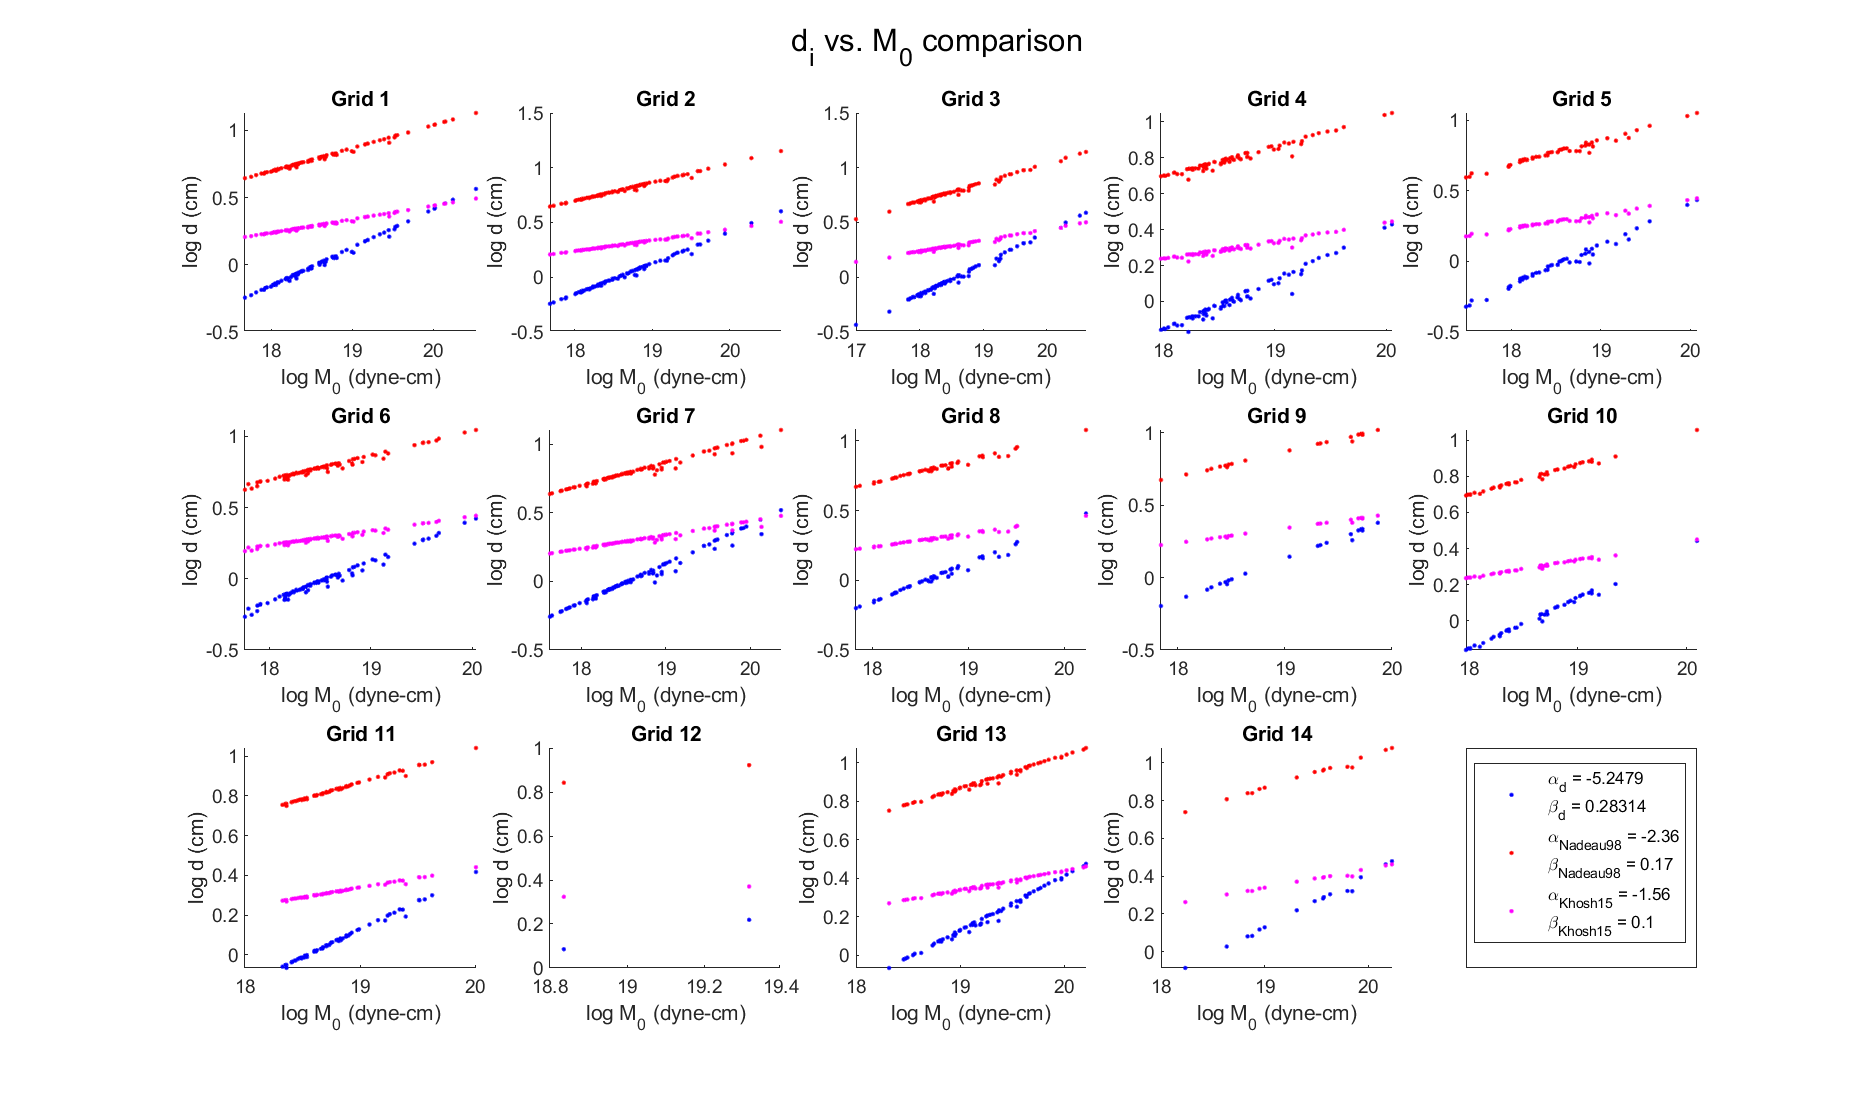
\includegraphics[width=10in]{slip_M0_comparison.png}%
    \caption{\label{fig:slip} Comparison of slip estimates obtained using three different calibrations \cite{nadeau98,khoshmanesh15}. Each point represents the average slip and seismic moment for one repeater sequence (i.e. family). Note that the removal of repeater event pairs with recurrence interval less than 0.1 years results in some grids (e.g. grid 12) having very few repeater sequences.}
\end{sidewaysfigure}

\begin{figure}
\centering
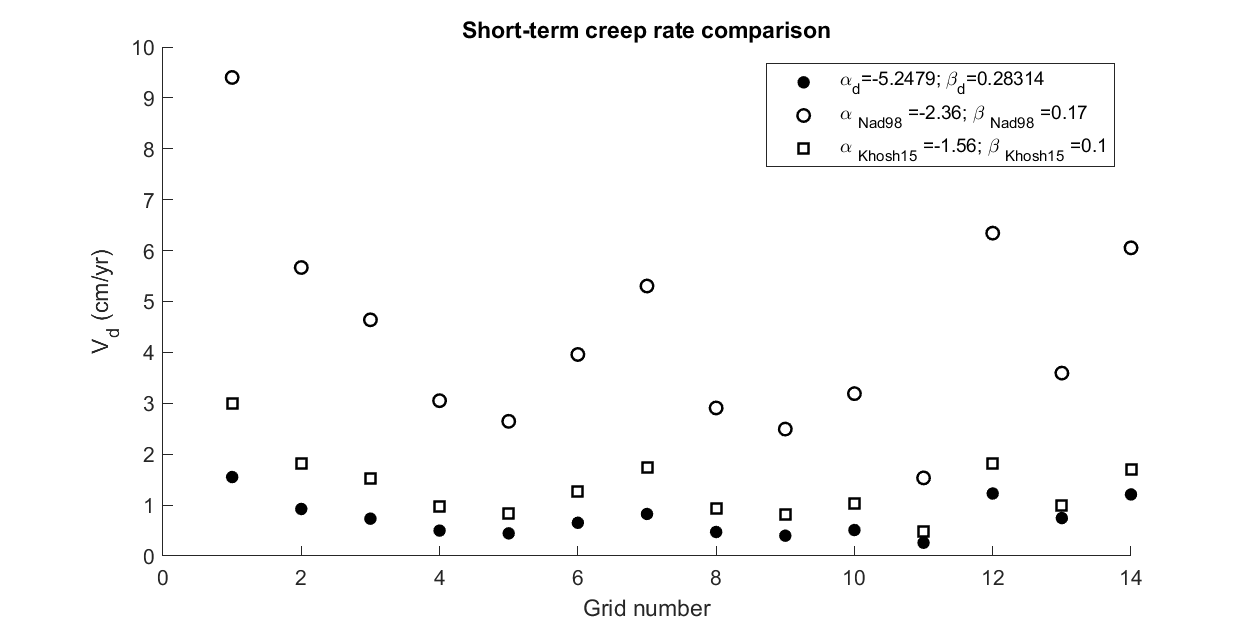
\includegraphics[width=6.5in]{short_term_creep.png}
\caption{\label{fig:Vd_short} Average short-term creep rates for each grid in the fault polygon. Short-term creep rates are not available from the USGS, and are thus not plotted here. The average creep rate from our parameters is 0.7467 cm/yr, compared to 4.3420 cm/yr using Nadeau's parameters and 1.3497 cm/yr using Khoshmanesh's. }
\end{figure}

\begin{figure}
\centering
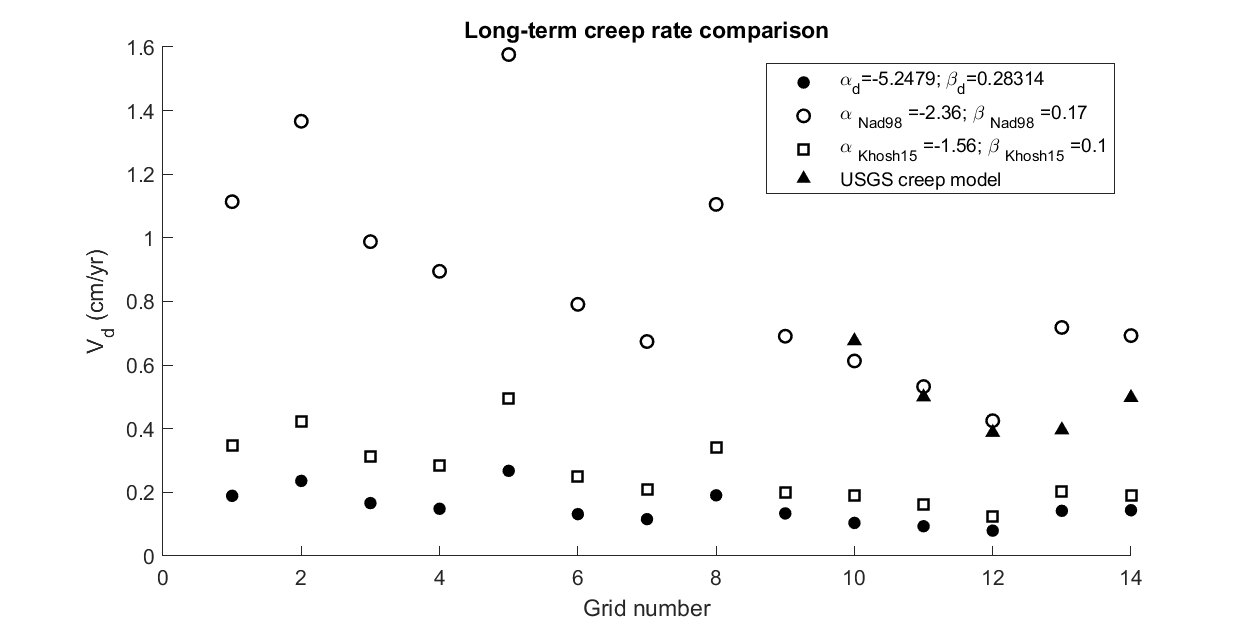
\includegraphics[width=6.5in]{long_term_creep.png}
\caption{\label{fig:Vd_long} Average long-term creep rates for each grid in the fault polygon. Both the slip parameters obtained by Khoshmanesh and this project produce significantly lower creep rates (averaged 0.2664 cm/yr and 0.1531 cm/year, respectively) than those obtained by the USGS \cite{johnson22}. The slip parameters obtained by Nadeau and Johnson \cite{nadeau98} produce creep rates closer to the available USGS estimates, with an average of 0.8703 cm/year. Further analysis is needed, either employing a more detailed creep data set or modifications to the parameter calibrations performed here (see text).}
\end{figure}

\section{Conclusion}
Our $\alpha_d$ and $\beta_d$ calibrations produced results inconsistent with available surface creep rates. Of the three calibrations tested, ours produced the lowest slip and creep rates, although it is worth noting the creep rates obtained from Khoshmanesh's $\alpha_d$ and $\beta_d$ constants were similar. 

Possible improvements to the $\alpha_d$ and $\beta_d$ calibrations involve fitting values to each grid, as opposed to applying one grid's calibration to the entire fault. The selection of grid thirteen, which has a high number of repeaters and thus a larger amount of creep, fails to represent grids with fewer repeaters (e.g. grids twelve and fourteen, Fig.\ref{fig:creep_locs}).
In addition to filtering based on recurrence interval, the identified repeaters should be filtered out based on a threshold covariance value (not calculated here), as done by Shakibay Senobari and Funning \cite{shakibay19}. Improvements can also be made to the filtering of events based on recurrence intervals. The effects of large earthquakes (e.g. increased repeater occurrences) were not taken into consideration in this process, and may have resulted in the lower slip and creep rate values through the exclusion of events.

\newpage
\bibliographystyle{acm}
\bibliography{refs}

\end{document}